\documentclass[tikz,border=5]{standalone}

\usepackage{mathdots}

\usetikzlibrary{calc}
\usetikzlibrary{decorations.pathreplacing}
\usetikzlibrary{scopes}

\begin{document}
  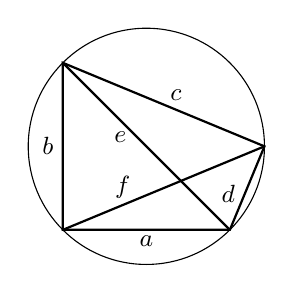
\begin{tikzpicture}
    \tikzset{font=\small}
    \begin{scope}[shift={(0,0)}]
      \draw (0,0) circle (1.5);

      \draw[thick]
        (  0:1.5) -- (135:1.5)
                  -- (225:1.5)
                  -- (315:1.5)
                  -- cycle;

      \draw[thick] (  0:1.5) -- (225:1.5);
      \draw[thick] (135:1.5) -- (315:1.5);

      \node (l01) at (270:1.20) {$a$};
      \node (l12) at (180:1.25) {$b$};
      \node (l23) at ( 60:0.75) {$c$};
      \node (l30) at (330:1.20) {$d$};
      \node (l02) at (160:0.35) {$e$};
      \node (l02) at (240:0.60) {$f$};
    \end{scope}
  \end{tikzpicture}
\end{document}
